\section{Irradiación solar}

	\subsection{Clasificaciones de la irradiancia}
			
		La irradiancia que recibe un objeto es clasificada de acuerdo a las interacciones por las que ese haz de luz pasó antes de llegar a dicho objeto.
		
		\begin{itemize}
			\item \textbf{Radiación directa:} Aquella que no tuvo interacción con otros cuerpos y que llega sin cambio de dirección.
			\item \textbf{Radiación difusa:} Aquella que sufrió algún choque con un cuerpo de la atmósfera, por ejemplo, la luz que atravesó una nube y fue difractada.
			\item \textbf{Radiación reflejada:} Aquella que proviene de la reflexión de la radiación directa.
		\end{itemize}
	
	\subsection{Propiedades espectrales de la radiación solar}
		
		Todas las radiaciones electromagnéticas viajan en el vacío con la misma rapidez ($\gls{c} = \qty{2.99792458e8}{\m\per\s}$) sin importar la fuente de emisión \cite{young_fisica_2009}, y todos los cuerpos que poseen temperatura por arriba de los 0 grados kelvin emiten radiación electromagnética derivada del movimiento vibracional de sus moléculas; las frecuencias emitidas y asociadas a esta vibración dan origen a la radiación térmica. Nótese que la luz no necesariamente tiene la misma energía a pesar de viajar a la misma rapidez.
		
		Cerca del \percent{99} de la potencia recibida por el sol está entre los \qtyrange{300}{2500}{\nm}. En las~\cref{fig:Espectro-radiación-solar,fig:Potencia-solar} notamos que de la irradiancia solar recibida, un aproximado del \percent{44} de la energía total corresponde al espectro visible mientras que un \percent{52} pertenece a la región del infrarrojo y el \percent{4} restante correspondería a la radiación ultravioleta \cite{weinstein_spectral_nodate}.
		
		\begin{figure}[H]
			\centering
			\begin{subfigure}{\linewidth}
				\centering
				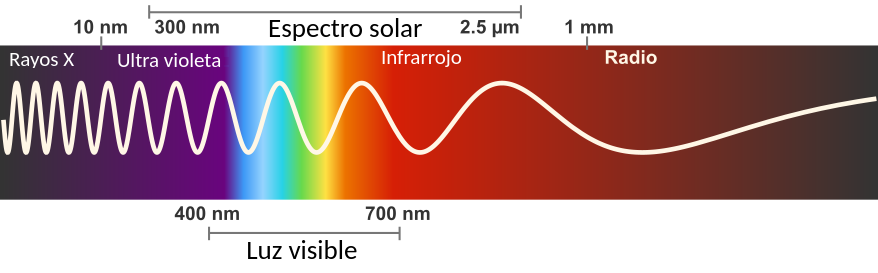
\includegraphics[width=\linewidth]{Marco-teórico/Espectro-radiación-solar.png}
				\caption{Espectro de radiación solar incidente sobre la Tierra}
				\label{fig:Espectro-radiación-solar}
			\end{subfigure}
			\begin{subfigure}{\linewidth}
				\centering
				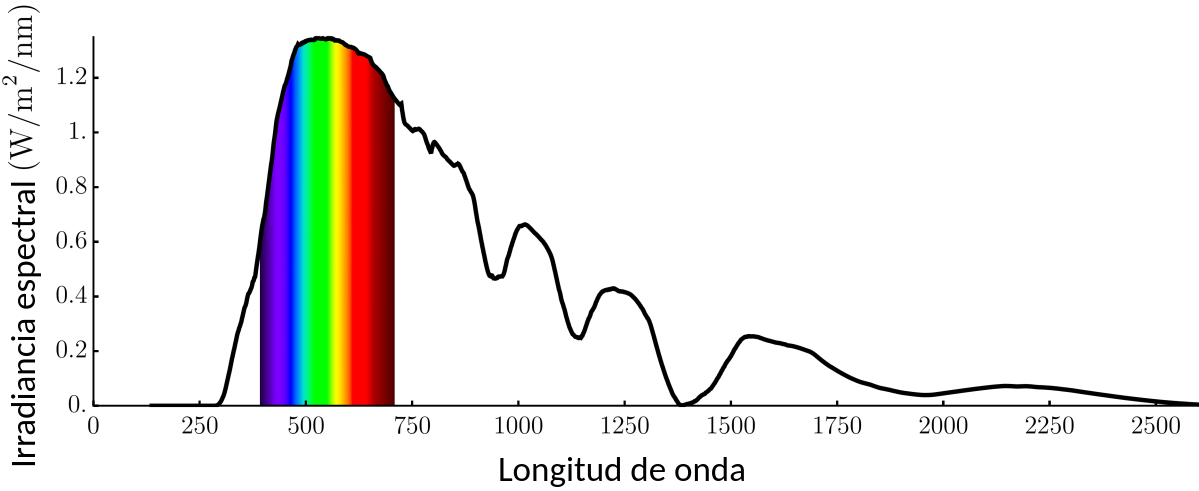
\includegraphics[width=\linewidth]{Marco-teórico/Potencia-solar.png}
				\caption{Potencia recibida del sol en la Tierra}
				\label{fig:Potencia-solar}
			\end{subfigure}
			\caption{Imágenes traducidas de \cite{weinstein_spectral_nodate}}
			\label{fig:solar-spectrum-brilliant}
		\end{figure}
		
%		Las longitudes de onda entre \qtyrange{700}{1e7}{\nm} son asociadas directamente al calor 
		
	
	\subsection{Irradiancia solar en la Tierra}
	
		El sol posee una temperatura superficial aproximada de \SI{5778}{\kelvin}, la cual emite calor en forma de radiación constantemente, de la cual, en el tope de la atmósfera terrestre se recibe un valor conocido como constante solar (\gls{G}) cuyo valor actualizado es de \SI{1360.8}{\watt\per\m\tothe{2}} $\pm$ \SI{0.5}{\watt\per\m\tothe{2}}. Sin embargo, no toda esa energía llega a la superficie terrestre~\cref{fig:atenuación-radiación-solar} debido a una serie de factores como el movimiento de rotación y traslación así como la inclinación de la Tierra, las condiciones climáticas y geográficas propias de la zona, del día  y de las interacciones a lo largo de su trayectoria por la atmósfera \cite{garcia_valladares_aplicaciones_2017}.
		
		\begin{figure}[H]
			\centering
			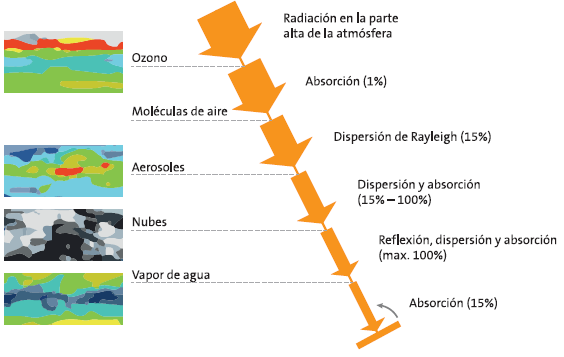
\includegraphics[width=\linewidth]{Marco-teórico/atenuación-radiación-solar.png}
			\caption{Atenuación de la radiación solar por su paso por la atmósfera}
			\label{fig:atenuación-radiación-solar}
			\floatfoot{Imagen obtenida de \cite{garcia_valladares_aplicaciones_2017}}
		\end{figure}
		
		
		
		
	
		
		
		